\documentclass{report}

\setlength{\textwidth}{150mm}
%\setlength{\textheight}{195mm}
\setlength{\oddsidemargin}{9mm}
%\setlength{\evensidemargin}{28mm}
%\setlength{\topmargin}{-10mm}


\usepackage[utf8]{inputenc}
\usepackage{graphicx}
\graphicspath{ {images/} }
\usepackage{caption}
\usepackage{subcaption}
\usepackage{wrapfig}

\begin{document}
\begin{titlepage}
\centering

\begin{figure}[t]

\includegraphics[scale=0.5]{images/urjc_logo.png}
\centering
\vspace{0.5cm} %Espacios despúes de la imagen
\end{figure}

{\scshape\Large Escuela Técnica Superior de Ingeniería de Telecomunicación \par}
\vspace{1cm}
{\scshape\Large Grado en Ingeniería en Sistemas de Telecomunicación \par}
\vspace{3cm}
{\bfseries\LARGE INTEGRACIÓN DE ROBOTS FÍSICOS EN LA PLATAFORMA KIBOTICS \par}
\vspace{3cm}
{\itshape\Large Trabajo Fin de Grado \par}
\vfill
{\Large Autor: }
{\Large David ValladaresVigara \par}
{\Large Tutores: }
{\Large Jose María Cañas Plaza y Julio Manuel Vega Pérez \par}
\vfill
{\Large Curso Académico 2019/2020 \par}
\end{titlepage} 

\renewcommand{\abstractname}{\Large Resumen}
\begin{abstract}



\end{abstract}

\setcounter{tocdepth}{3} %Para que aparezcan las subsubsection{}
\renewcommand{\contentsname}{Índice general}
\tableofcontents
\clearpage

\renewcommand{\listfigurename}{Índice de figuras}
\listoffigures

\renewcommand{\listtablename}{Índice de tablas}
\listoftables

\renewcommand{\chaptername}{Capítulo}
\chapter{Introducción}

En este capítulo se introducen las aplicaciones de la robótica para el ambiente educativo y las motivaciones que han llevado al desarrollo del Trabajo de Fin de Grado (TFG). Este TFG se ha desarrollado dentro de la plataforma Kibotics para tratar de mejorar la integración sobre robots reales.

\section{Robótica educativa}

La robótica es la ciencia que estudia el diseño y la construcción de máquinas que permiten realizar y facilitar tareas desempeñadas por el ser humano (Quiroga, 2018). Actualmente puede considerarse una de las áreas de las Tecnologías de la Información y Comunicación (TIC) con más auge, pues cada vez es más habitual el uso de robots limpiadores (p. ej. Roomba de iRobot) (Figura 1.1), asistentes virtuales (p. ej. Alexa de Amazon) o el empleo de brazos robóticos en las cadenas de montaje de las industrias. Por ello, resultan muy beneficiosos en el sector industrial y el de servicios (Salamanca, Barrera y Pérez, 2010).
\\
\begin{figure}
  \centering
    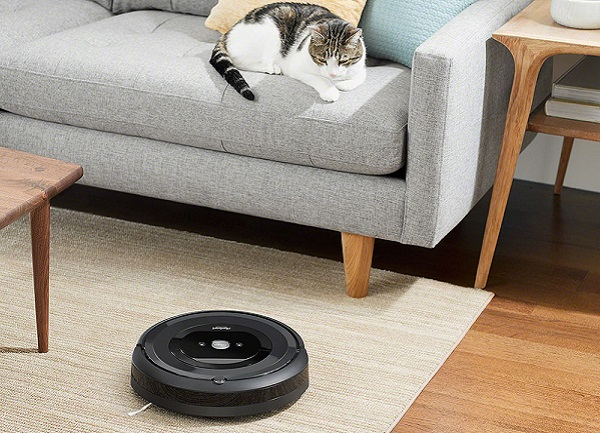
\includegraphics[width=0.4\textwidth]{images/romba.png}
  \caption{Robot aspirador modelo Roomba®}
  \label{Roomba}
\end{figure}
\\

Sin embargo, desde los años sesenta aumentó el interés por introducir la robótica también en el ámbito educativo, creando así la “Robótica educativa” o “Robótica pedagógica”. Se define como una disciplina que permite concebir, diseñar y desarrollar robots educativos para que las personas se puedan iniciar pronto en el mundo de la ciencia y tecnología (Ruiz-Velasco, García y Rosas, 2007). Al combinar diferentes áreas del conocimiento, se ha convertido en una herramienta novedosa que puede utilizarse en las primeras etapas de la educación de los niños y niñas ayudando a potenciar su desarrollo integral (Quiroga, 2018) y que, además, permite que los estudiantes adquieran otras competencias, como la socialización, la creatividad,  la iniciativa y el pensamiento lógico (Bravo y Forero, 2012).
\\

Los orígenes de la robótica educativa se remontan al siglo XX con la teoría constructivista de Jean Piaget, la cual indica que el conocimiento se construye activamente en la mente del estudiante. Esto coincide con la pedagogía del construccionismo de Seymour Papert donde, además, se afirma que lo que construye el individuo debe ser tangible y con un significado personal para él. Algunos desarrollos de la robótica educativa se basan en esta última (González y Jiménez, 2009).
\\

La robótica educativa, por tanto, se considera una herramienta paralela a las asignaturas tradicionales al volverlas más atractivas e integradoras para los estudiantes (Quiroga, 2018). Con ello, ayuda a los alumnos a construir conceptos y a hacer una interpretación personal de la realidad (Salamanca, Barrera y Pérez, 2010).
\\

\subsection{Ejemplo de Metodología para la enseñanza}

Una de las metodologías para llevar a cabo un proceso de trabajo de robótica es la de las cuatro palabras de Báez et al. (2011), representadas en la Figura 1.2. La primera de ellas es “imaginar” porque los estudiantes piensan y debaten sobre dispositivos que pueden ser útiles para resolver un problema o facilitar un trabajo, lo que favorece al pensamiento creativo. A continuación, encontramos la palabra “diseñar”, que les permite crear el artefacto que han imaginado consiguiendo una conexión entre el mundo físico y la imaginación. La tercera es “construir”, que se basa en el montaje de los dispositivos que han diseñado los miembros del grupo de trabajo, por lo que favorece la cooperación y el trabajo manual. La última palabra del proceso es “programar” o dotar de inteligencia a los dispositivos montados a través de un ordenador, mejorando el pensamiento lógico, la autopercepción y el análisis espacial.
\\
\begin{figure}[h!]
  \centering
    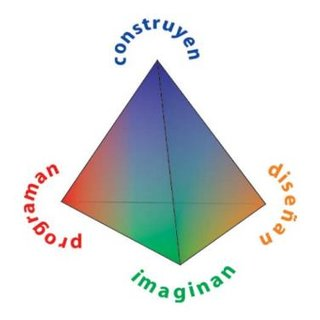
\includegraphics[width=0.4\textwidth]{images/metodologia.png}
  \caption{Las cuatro palabras de la Robótica educativa (Báez et al., 2011).}
  \label{Metodologia}
\end{figure}
\\

\subsection{Aumento de la implantación de la robótica en las aulas}

En la última década, la robótica ha adquirido mucha importancia en un gran número de países (Quiroga, 2018), y cada vez genera más interés implantarla en las aulas (Salamanca, Barrera y Pérez, 2010).
\\

Esto se debe a que aporta muchos beneficios en el proceso de enseñanza-aprendizaje de asignaturas difíciles (Moreno et al., 2012). También es más frecuente la creación de robots para la vida cotidiana, lo que despierta el interés de las personas en ellos (Quiroga, 2018). Además, la existencia de lenguajes de programación orientados a alumnos de menor edad (p. ej. Scratch - Figura 1.3) y la mayor disponibilidad de kits de robótica educativa en el mercado los ha convertido en productos ideales para la iniciación en este campo.
\\
\begin{figure}[h!]
  \centering
    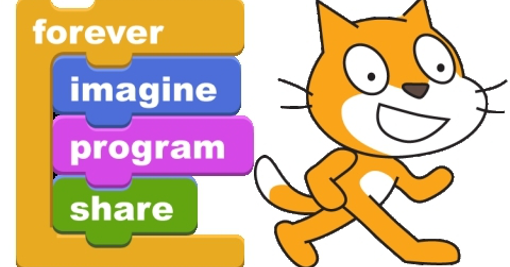
\includegraphics[width=0.3\textwidth]{images/logo_scratch.png}
  \caption{Scratch}
  \label{Scratch}
\end{figure}
\\

Algunos de los robots existentes en el mercado orientados a ese aprendizaje en la robótica son:
\begin{itemize}
	\item \textbf{Mbot}. Diseñado por la empresa MakeBlock y basado en Arduino Uno, una placa electrónica que contiene un microcontrolador programable.
		\begin{figure}[h!]
  			\centering
   			 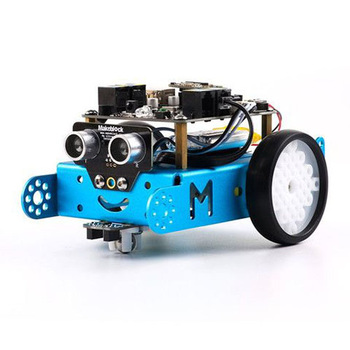
\includegraphics[width=0.3\textwidth]{images/mbot.png}
 			 \caption{Mbot}
 			 \label{Mbot}
		\end{figure}
	\item \textbf{Tello de Ryze Dji }. Es un pequeño dron pensado para que los niños y adultos aprendan su manejo de forma sencilla.
		\begin{figure}[h!]
  			\centering
   			 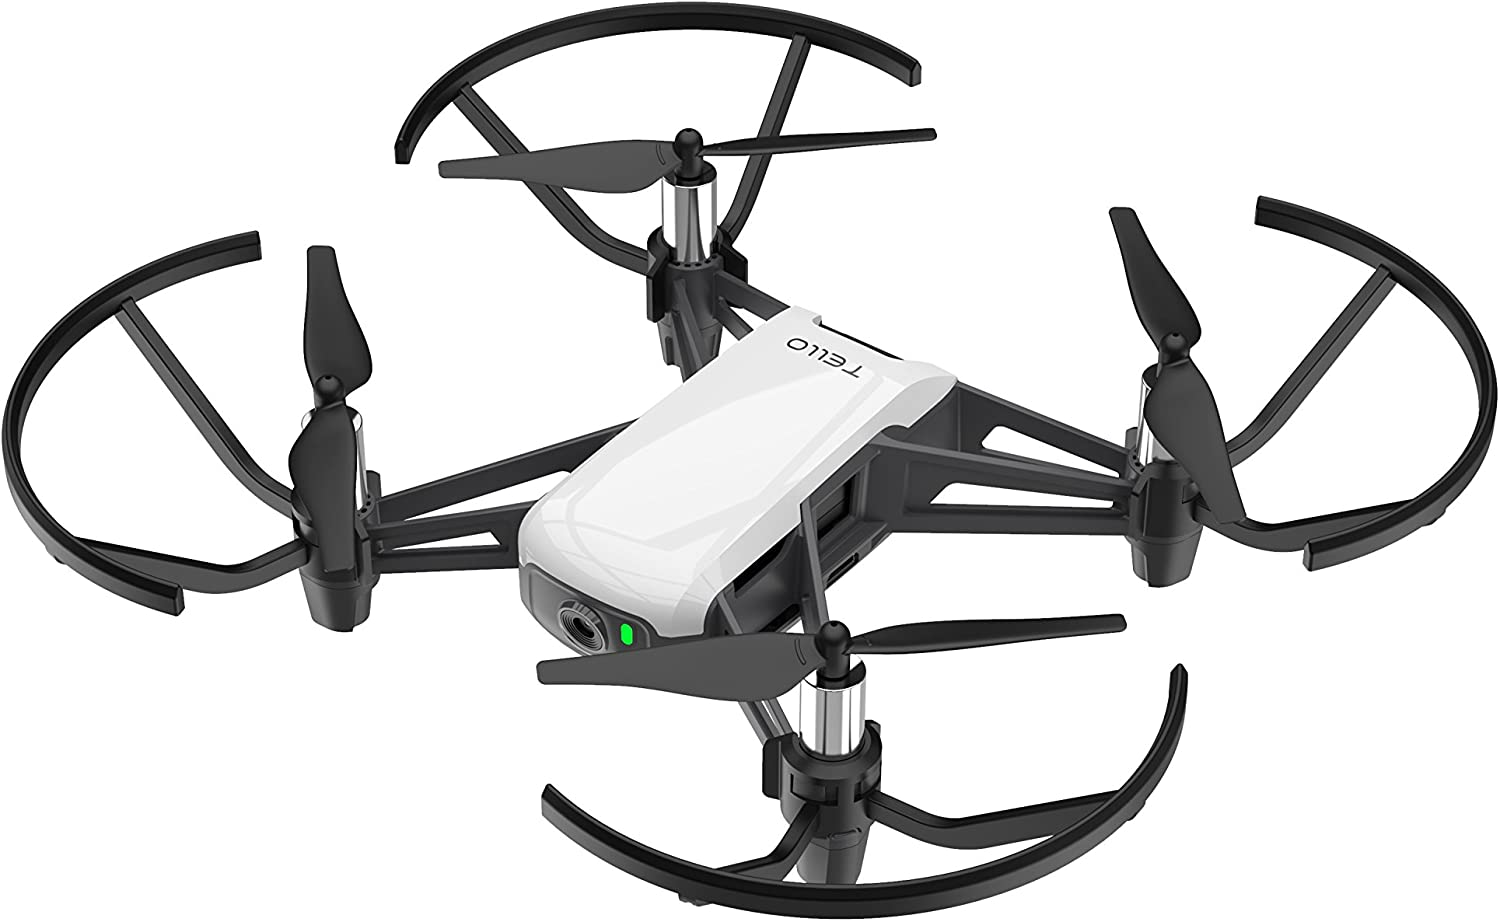
\includegraphics[width=0.3\textwidth]{images/tello.png}
 			 \caption{Tello}
 			 \label{Tello}
		\end{figure}
	\item \textbf{GopiGo3}. Es un robot con forma de coche creado por Dexter Industries, se caracteriza porque su controladora es una RaspberryPi 3, un mini-ordenador de bajo conste que le dota de una gran inteligencia.
		\begin{figure}[h!]
  			\centering
   			 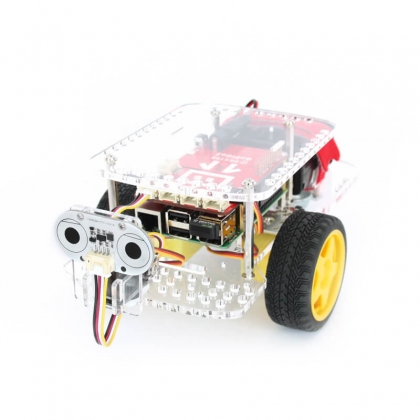
\includegraphics[width=0.3\textwidth]{images/gopigo.png}
 			 \caption{GopiGo3}
 			 \label{GopiGo3}
		\end{figure}
\end{itemize}

Por último, existen aplicaciones y páginas web de programación robótica que facilitan la creación de programas para los robots, como pueden ser Mblock (desarrollada por la empresa MakeBlock y basada en Scratch 3), Bitbloq (creada por la empresa bq, que utiliza bloques para realizar los programas y es compatible con la placa arduino) o Kibotics (llevada a cabo por JdeRobot).
\\

\section{Kibotics}

Kibotics (Figura 1.7) es un entorno web utilizado para la docencia en los campos de robótica, programación y áreas STEM (acrónimo de Science, Technology, Engineering and Mathematics).
\\
\begin{figure}[h!]
  \centering
    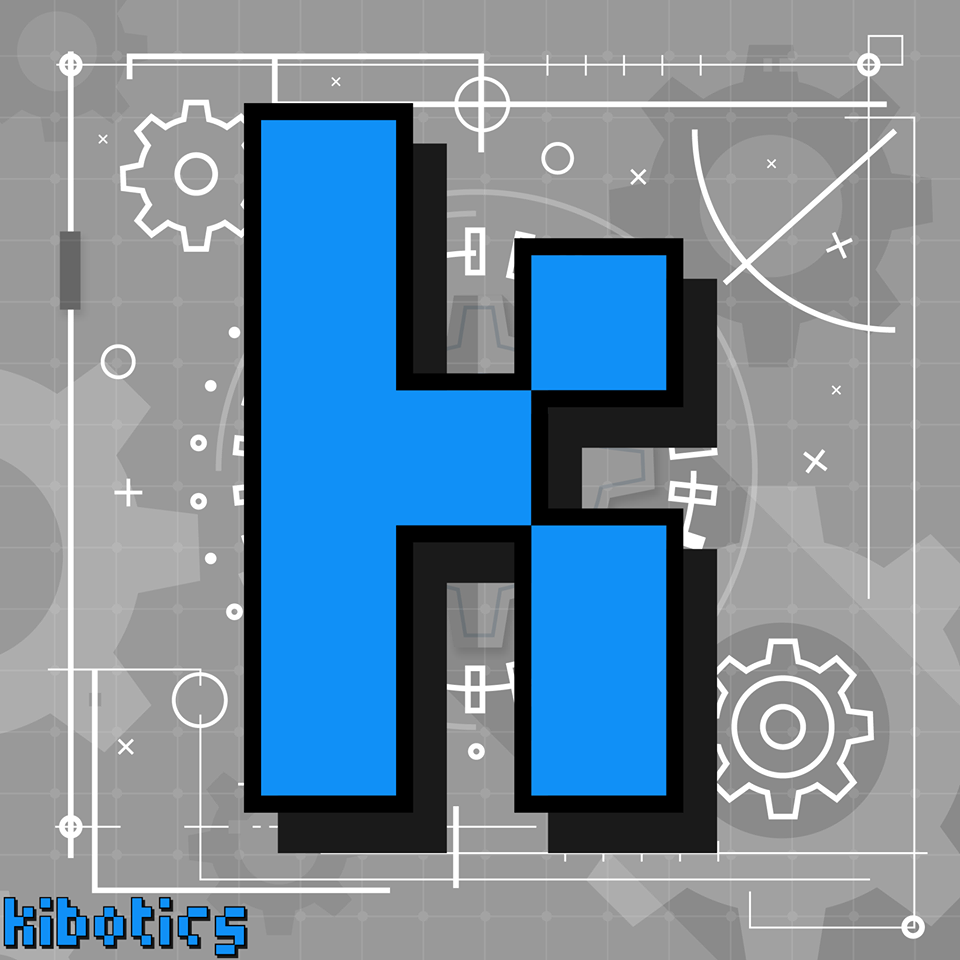
\includegraphics[width=0.3\textwidth]{images/logo_kibotics.png}
  \caption{Logo de Kibotics}
  \label{Logo de Kibotics}
\end{figure}
\\


Ayuda a los alumnos a iniciarse en el mundo de la robótica y la programación de forma sencilla y práctica.
\\

\subsection{Lenguajes soportados en Kibotics}

La plataforma proporciona, actualmente, ejercicios para dos lenguajes de programación. El primero de ellos es Blockly, que fue desarrollado por Google y es muy similar a Scratch. Está orientado para alumnos de menor edad por ser un lenguaje de programación visual basado en una interfaz de bloques que se pueden encajar como si fuera un puzle. Su uso en colegios e institutos es cada vez mayor, ya que está diseñado para que la iniciación al mundo de la programación sea sencilla, divertida y creativa.
\\

Los procedimientos utilizados en la programación de Blockly en Kibotics se clasifican en:
\begin{itemize}
	\item \textit{Serie} : ordenación de los bloques creando una secuencia lógica.

	\item \textit{Bucles}: proporcionan la posibilidad de introducir repeticiones sobre una secuencia deseada.
		
	\item \textit{Variables}: aquellas estructuras de datos en las que se pueden almacenar información a lo largo de la ejecución de un programa.
	
	\item \textit{Operadores lógicos}: devuelve un resultado de verdadero o falso en función de si se cumple o no una determinada condición.
	
	\item \textit{Bloques condicionales}: permiten decidir qué camino lógico tomar en base a una operación lógica.
	
	\item \textit{Operador matemático}: aquellos bloques que permiten realizar una operación matemática.
	
	\item \textit{Robot Api}: se proporciona una interfaz con los actuadores y sensores disponibles para un determinado robot, facilitando así su programación.
\end{itemize}

El segundo es Python, enfocado para alumnos mayores. Constituye uno de los lenguajes de programación con más popularidad en la actualidad según el Índice de Popularidad de Lenguajes de Programación (PYPL PopularitY of Programming Language index, 2020). Es multiparadigma, multiplataforma, gratuito, posee un tipado dinámico e interpretado, es decir, no necesita que un compilador lo procese. Estas características, además de tener una sintaxis legible, permiten un aprendizaje más sencillo que con otros lenguajes de programación como Blockly (Figura 1.8).
\\
\begin{figure}[h!]
  \centering
    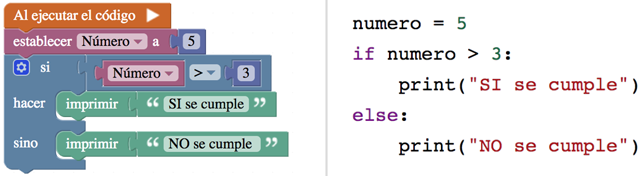
\includegraphics[width=1\textwidth]{images/blockly-vs-python.png}
  \caption{Comparación del mismo código escrito en Blockly (izquierda) y Python (derecha)}
  \label{Comparación del mismo código escrito en Blockly y Python}
\end{figure}
\\

En Kibotics se proporciona una variedad de ejercicios para poner en práctica la programación en Python en diferentes robots. Además, para facilitar el manejo con ellos, se han desarrollado librerías que proporcionan funciones para interactuar con los actuadores y sensores de los robots disponibles. Por ejemplo, en la Figura 1.9 se indican algunas funciones disponibles para el manejo del Dron “Tello”.
\\
\begin{figure}[h!]
  \centering
    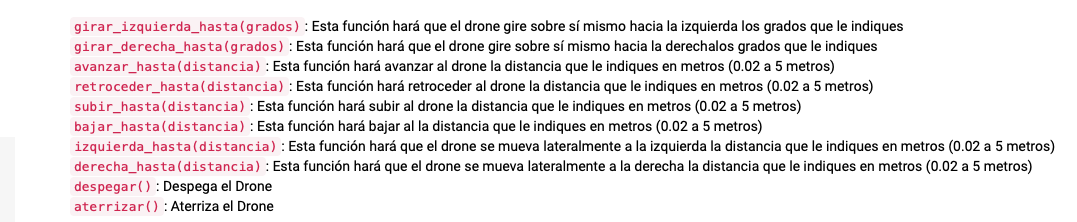
\includegraphics[width=1.1\textwidth]{images/api.png}
  \caption{Funciones disponibles para el Dron “Tello”.}
  \label{Funciones disponibles para el Dron “Tello”.}
\end{figure}
\\

\subsection{Tipos de Robots}

No existe una definición única universal para la palabra “robot”. Por ejemplo, la Real Academia Española (RAE) determina que es una “máquina o ingenio electrónico programable, capaz de manipular objetos y realizar operaciones antes reservadas solo a las personas” (RAE, 2020). También se define como un “sistema compuesto por mecanismos que le permiten hacer movimientos y realizar tareas específicas, programables y eventualmente inteligentes, valiéndose de conceptos de otras áreas del conocimiento” (Salamanca, Barrera y Pérez, 2010).
\\

Un robot se compone, principalmente, de las siguientes partes:
\begin{itemize}
	\item \textit{Esqueleto}. Encargado de soportar los componentes que forman al robot.

	\item \textit{Controladora}. Encargada de procesar los datos obtenidos de los sensores, tomar decisiones y enviar las órdenes a los actuadores.
		
	\item \textit{Sensores o receptores}. Miden magnitudes físicas y las transforman a magnitudes eléctricas. Existen dos tipos, por un lado, están los encargados del entorno que les rodea y, por otro, los del estado interno. Ejemplos de sensores son los infrarrojos, de proximidad, ultrasonido, etc.
	
	\item \textit{Actuadores}. Encargados del movimiento del robot mediante las órdenes recibidas de la controladora.
\end{itemize}

En Kibotics se distinguen dos tipos de robots con los que se puede interactuar: los robots simulados (p. ej. Drone Tello, Mbot, Pibot) y los robots físicos o reales (p. ej. Pibot).
\\

Los robots simulados son robots virtuales que emulan el comportamiento de un robot real, permitiendo al usuario interactuar con él como si fuera uno real (Figura 1.10). Esto se fundamenta en la idea de Robert E. Shannon de simulación como “un proceso de diseñar un modelo de un sistema real y llevar a termino experiencias con él, con la finalidad de comprender el comportamiento del sistema o evaluar nuevas estrategias para el funcionamiento del sistema” (Shannon, 1998).  Al trabajar con ellos, no se necesita su presencia física, se crea una interacción más segura y se puede experimentar con situaciones más complejas o con las que no se posee información.
\\
\begin{figure}[h!]
  \centering
    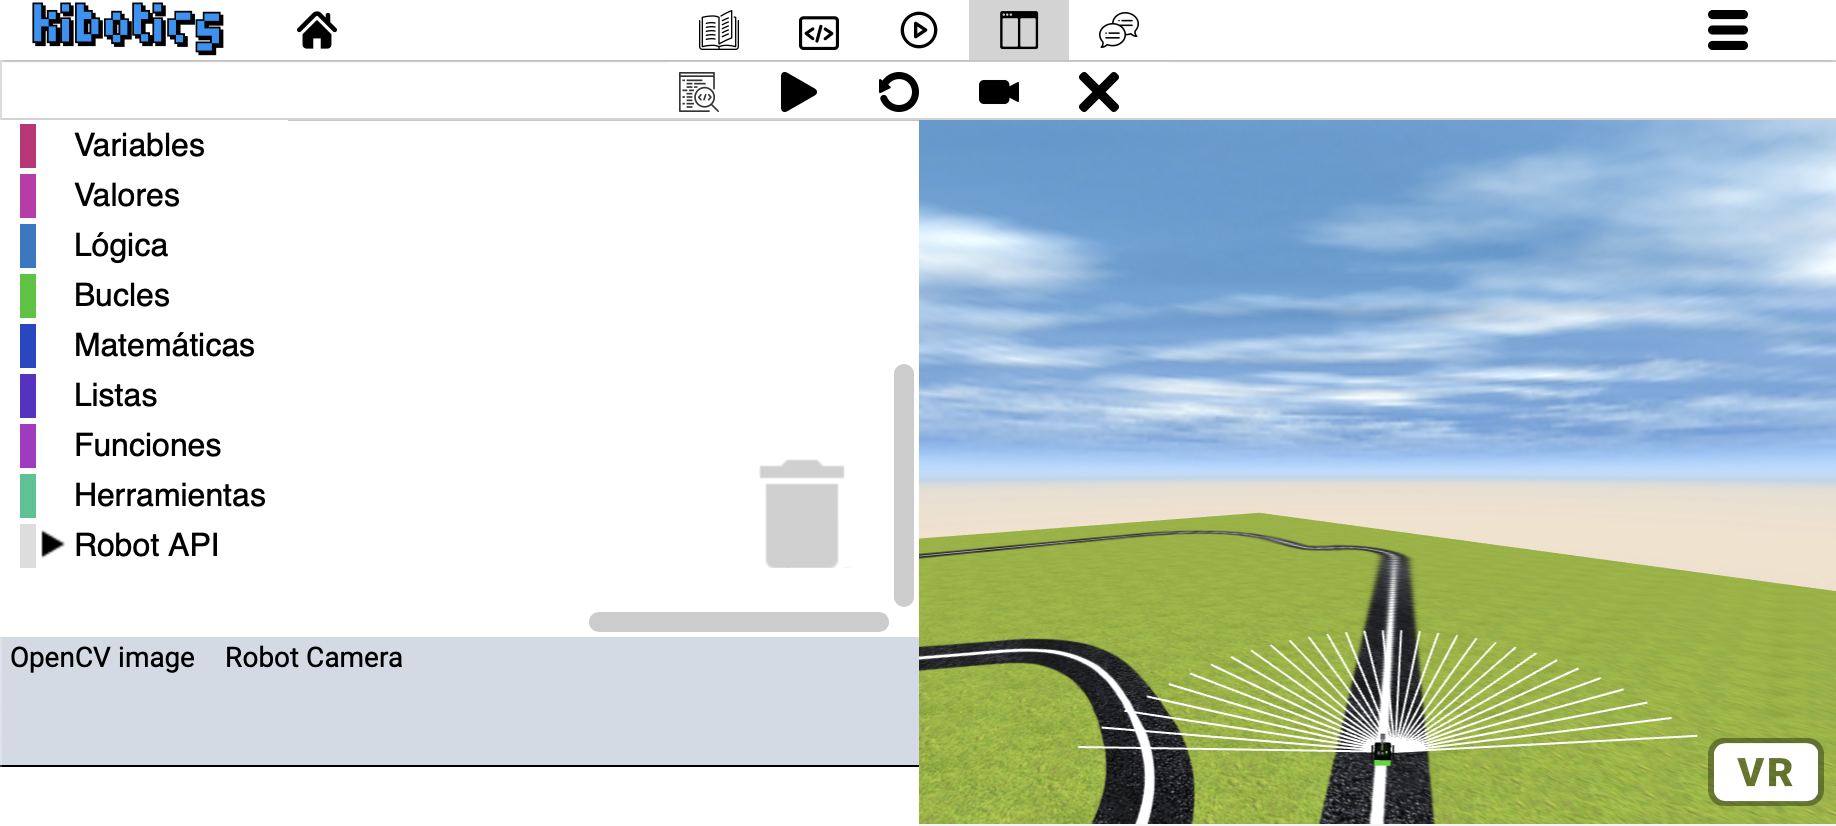
\includegraphics[width=0.9\textwidth]{images/simulado.png}
  \caption{Ejemplo de Robot simulado en Kibotics}
  \label{Ejemplo de Robot simulado en Kibotics}
\end{figure}
\\

En cuanto a los robots físicos o reales, desde Kibotics se da soporte para el desarrollo de programas y envíos sobre algunos de ellos, por ejemplo, para el Pibot mencionado anteriormente. Con ello, se pretende facilitar este proceso de comunicación, que en muchas ocasiones puede no ser sencillo.
\\

En este punto recae la motivación principal para este TFG, que consiste en proporcionar soporte para el uso sobre robots reales, como Mbot, Tello y Gopgio, aunque se hablará más en detalle en el capítulo dos.

\chapter{Objetivos}

\section{Objetivos}
\section{Metodología}
\section{Requerimientos}

\chapter{Herramientas}

\chapter{Mbot}

\chapter{Dron Tello}

\chapter{GopiGo3}

\chapter{Conclusiones}
\subsection{Conclusiones}
\subsection{Líneas futuras}

\chapter{Bibliografía}

Báez, M.; Bongiovanni, P.; Castrillejo, D.; García, J. M.; Leal, D.; Levis, D.; Lugo, M. T.; Maguregui, C.; Ochoa, G.;  Peña-López, I.; Pisano, R.; Rabajoli, G.; Rivoir, A.; Sansberro, F.; Turner, N.; Vacca, A. M.; Vaillant, D. (2011). El modelo CEIBAL. Nuevas tendencias para el aprendizaje. Uruguay: CEIBAL - ANEP.
\\

Bravo, F. Á.; Forero, A. (2012). La robótica como un recurso para facilitar el aprendizaje y desarrollo de competencias generales. \textit{Teoría de la Educación. Educación y Cultura en la Sociedad de la Información} 13(2): 120-139.
\\

González, J. J.; Jiménez, J. A. (2009). La robótica como herramienta para la educación en ciencias e ingeniería. \textit{IE Comunicaciones: Revista Iberoamericana de Informática Educativa} 10: 31-36.
\\

Curso de iniciación a Python en Raspberry Pi. (2020). Recuperado 12 de septiembre de 2020, de Asociación Programo Ergo Sum website: https://www.programoergosum.com/cursos-online/raspberry-pi/244-iniciacion-a-python-en-raspberry-pi/que-es-python
\\

Moreno, I.; Muñoz, L.; Serracín, J. R.; Quintero, J.; Patiño, K. P.; Quiel, J. (2012).\textit{ La robótica educativa, una herramienta para la enseñanza-aprendizaje de las ciencias y las tecnologías. Teoría de la Educación. Educación y Cultura en la Sociedad de la Información} 13(2): 74-90.
\\

PYPL PopularitY of Programming Language index. (2020). Recuperado 15 de septiembre de 2020, de PYPL PopularitY of Programming Language website: http://pypl.github.io/PYPL.html
\\

Quiroga, L. P. (2018). \textit{La robótica: otra forma de aprender. Revista Educación y Pensamiento} 25(25): 51-64
\\

REAL ACADEMIA ESPAÑOLA: \textit{Diccionario de la lengua española}, 23.ª ed., [versión 23.3 en línea]. <https://dle.rae.es> [12 de septiembre de 2020].
\\

Ruiz-Velasco, E.; García, J. V.; Rosas, L. A. (2007). \textit{Robótica pedagógica virtual para la inteligencia colectiva}. México: Universidad Nacional Autónoma de México.
\\

Salamanca, M. L.; Barrera, N.; Pérez, W. J. (2010). \textit{Uso de la robótica educativa como herramienta en los procesos de enseñanza}. Ingeniería Investigación y Desarrollo: I2+D 10(1): 15-23.
\\

Shannon, R. E. (1998, diciembre 13-16). \textit{Introduction to the art and science of simulation}. In 1998 Winter Simulation Conference. Doi: 10.1109/WSC.1998.744890

\end{document}
